UvA Bird Tracking System\footnote{\url{http://www.uva-bits.nl/} } is a research 
project that studies the behavior of
birds. 
In contrast to some other birds that are being tracked the Sea Gull flies above the 
sea where it is a lot harder to watch and see what it is doing. We have data available
collected by a small device (see figure \ref{fig:gpsDevice}) that can be attached to 
the back of a bird. 

\begin{figure}
    \center
    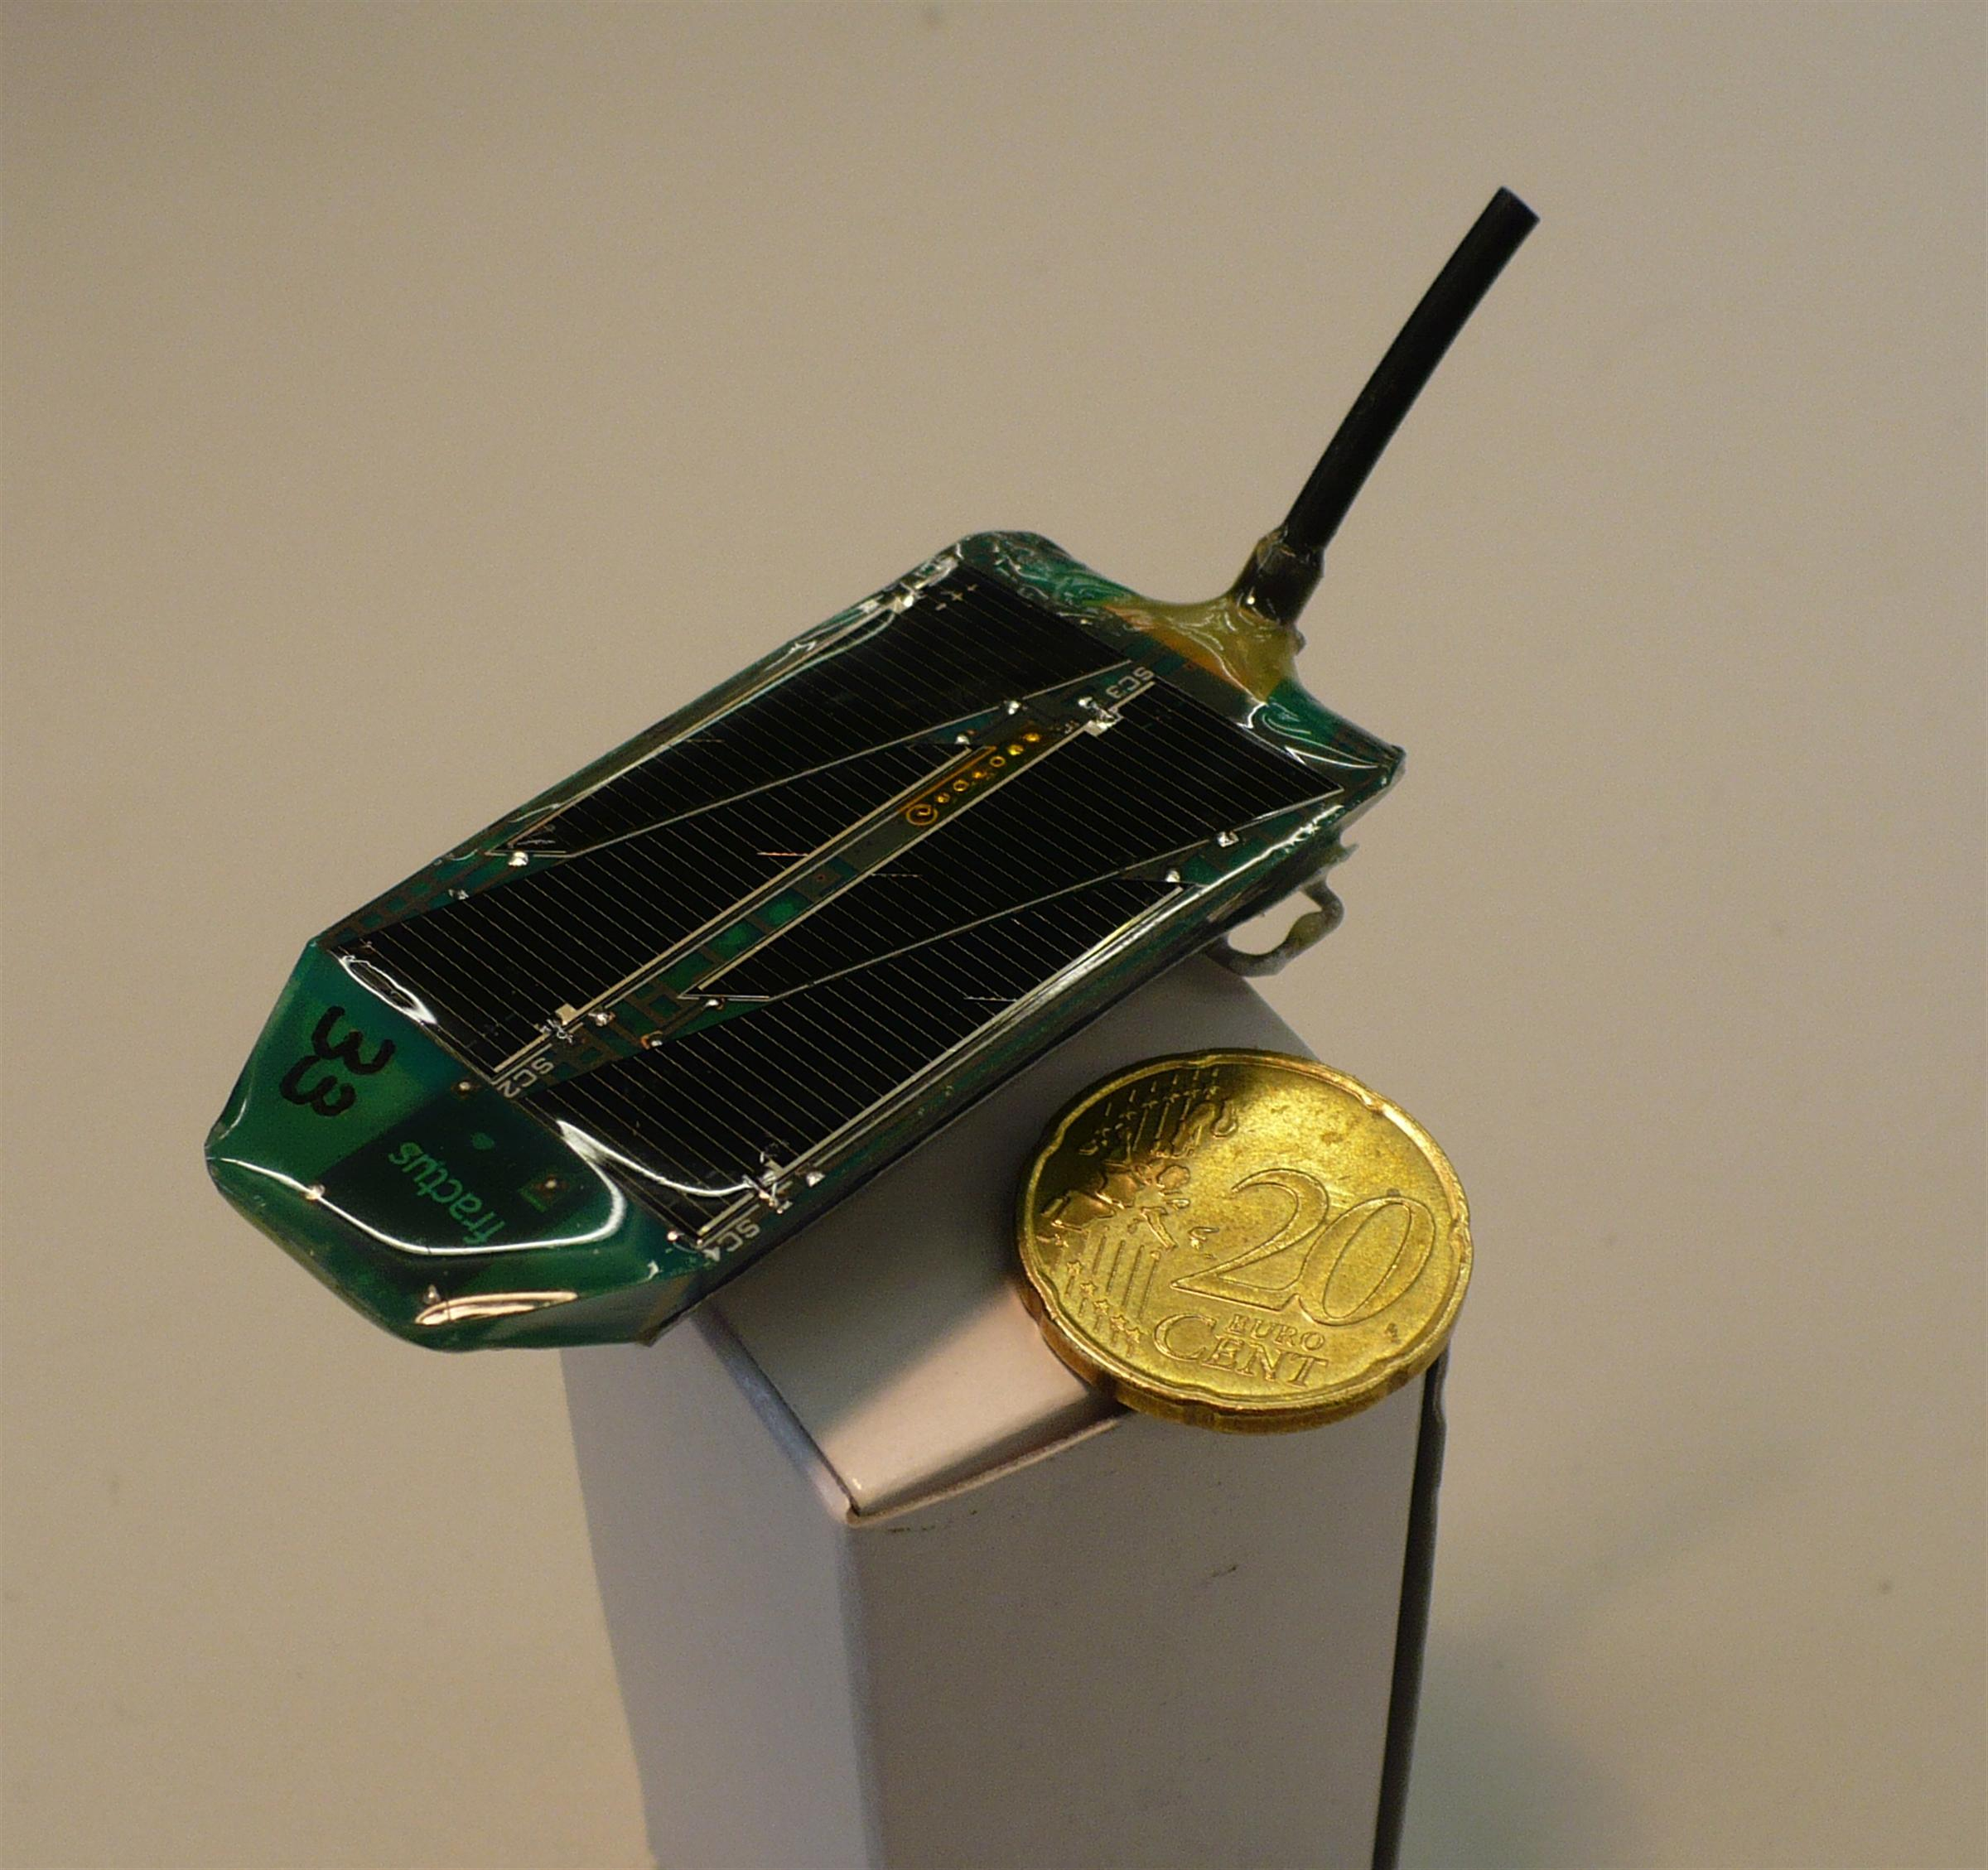
\includegraphics[width=7cm]{device}
    \caption{A small GPS device that can also transmit accelerometer data and some other
information}
    \label{fig:gpsDevice}
\end{figure}

The data, which consists of thousands of data points, is hard to read and to annotate. 
There are tools that can rewrite the data to a format that can be read by Google Earth. 
Viewing this data in Google Earth is a bit helpful to get a general idea of what such 
a gull might be doing but it does not allow for easy manipulation of the data. 

During four weeks we worked to preprocess, cluster, annotate
and lastly: classify the data. 

% perhaps more about the (other) research goals

